\chapter{Preliminaries}
\label{chapterlabel2}

\section{U-Net}
U-Net\cite{ronnebergerUNetConvolutionalNetworks2015} is commonly refers as a U-shaped encoder-decoder residual network architecture. It is originally developed for image segmentation in biomedical image processing (see figure \ref{fig:unet_arch}) based on a previous fully convolutional network study\cite{longFullyConvolutionalNetworks2015}. It is a popular approach in many vision tasks.

\begin{figure}
    \centering
    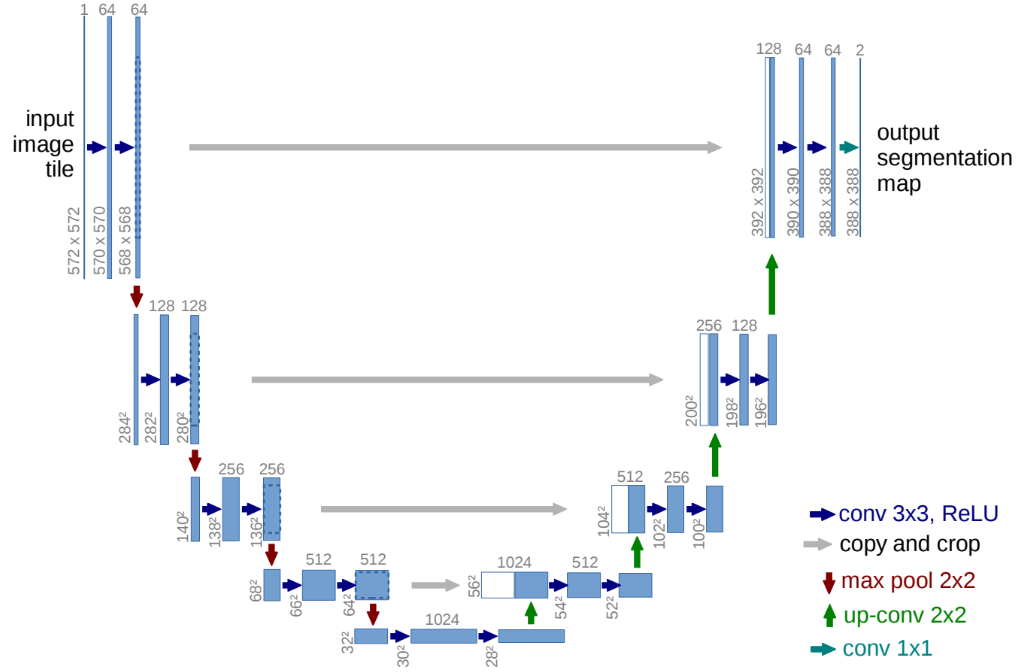
\includegraphics[width=0.75\textwidth]{images/preliminary/unet_arch.png}
    \caption{U-Net architecture. Light blue box corresponds to multi-channels features; blue arrow is 3x3 convolution with ReLU; gray arrow is copy and crop operations, more commonly known as skip/residual connection; red arrow is 2x2 max pooling; green arrow is 2x2 up convolution or interpolation; and light blue arrow is 1x1 convolution for feature reduction.\cite{ronnebergerUNetConvolutionalNetworks2015}} 
    \label{fig:unet_arch}
\end{figure}

The first half of the network consists of a number of encoder block. Each consists of a convolutional block followed by a ReLU activation and max pooling. Each block halves the size of feature map. The second half is similar to the first half, except it doubles the size of feature map at each decode block. The output of the corresponding encoder block is given as additional input to the decoder network, this operation is known as skip/residual connection.

Some implementation adds a batch normalization between the convolution layer and the ReLU layer, in attempts to reduces internal covariance shift and improve training stability. Dropout layer may also added after ReLU as a form of regularization to improve generalization of the network.

\section{GAN}

GAN stands for Generative Adversaial Network\cite{goodfellowGenerativeAdversarialNetworks2014a}, it is a machine learning framework where two networks simultaneously compete and learns from each other in the form of two-players, zero sum game. The network consists of a generator $\mathcal{G}$ tries to mimic the target and a discriminator $\mathcal{D}$ tries to distinguish between real and generated input. This training framework is commonly used in computer vision tasks to generate high quality images.

Major challenges exists in training GAN, it can fail easily due to various reasons such as mode-collapse (see appendix \ref{app:ml:mode_col}), vanishing gradient (see appendix \ref{app:ml:van_grad}), non-convergence (see appendix \ref{app:ml:non_conv}), instability, inappropriate design (e.g. under/overpowered discriminator, use of loss and optimization algorithm, etc.). Therefore a number of variations are proposed to improve it, and they are commonly adopted in most model describe in this paper.


\subsection{Wasserstein GAN}

\subsection{WGAN-GP}

\subsection{cGAN}

\section{ResNet}

\subsection{ResNeXt}

\section{Pix2pix}

\section{Pixel Shuffle}
